\documentclass[12pt, titlepage]{article}

\usepackage[margin=1in]{geometry}
\usepackage{booktabs}
\usepackage{tabularx}
\usepackage{longtable}
\usepackage{multirow}
\usepackage{float}
\usepackage{enumitem}
\usepackage{tikz}
\usetikzlibrary{arrows.meta, positioning}
\usepackage{xurl}
\usepackage{hyperref}
\hypersetup{colorlinks, linkcolor=red, urlcolor=blue, citecolor=blue}

\newcommand{\progname}{Natural Control}
\newcommand{\todo}[1]{\par\medskip\noindent\fbox{\parbox{0.95\linewidth}{\textbf{TODO (team):} #1}}\par\medskip}

\newcounter{acnum}
\newcommand{\actheacnum}{AC\theacnum}
\newcommand{\acref}[1]{AC\ref{#1}}
\newcounter{ucnum}
\newcommand{\uctheucnum}{UC\theucnum}
\newcommand{\ucref}[1]{UC\ref{#1}}
\newcounter{mnum}
\newcommand{\mthemnum}{M\themnum}
\newcommand{\mref}[1]{M\ref{#1}}

\begin{document}

\title{Module Guide for \progname{}\\[4pt]\large Design Document Revision -1 (draft)}
\author{Team 7: Aaron Loh, Curtis Vos, Kevin Kim, Lucas DeBoer}
\date{November 11, 2026}
\maketitle

\pagenumbering{roman}

\section{Revision History}

\begin{tabularx}{\textwidth}{p{3cm}p{2cm}X}
\toprule
\textbf{Date} & \textbf{Version} & \textbf{Notes}\\
\midrule
2026-11-11 & 0.1 & First draft, written from the simple POC in the team's prototype repository.\\
\bottomrule
\end{tabularx}

\section{Reference Material}

\subsection{Abbreviations and Acronyms}

\begin{tabularx}{\textwidth}{lX}
\toprule
\textbf{Symbol} & \textbf{Description}\\
\midrule
AC & Anticipated change\\
AI & Artificial intelligence; here, the language model that chooses which tool to use\\
FR, NFR & Functional and non-functional requirement, as numbered in the SRS\\
M & Module\\
MG & Module Guide\\
MIS & Module Interface Specification\\
POC & Proof of concept\\
SRS & Software Requirements Specification\\
STT, TTS & Speech to text, text to speech\\
UC & Unlikely change\\
\bottomrule
\end{tabularx}

\subsection{Services and Tools}

\begin{tabularx}{\textwidth}{lX}
\toprule
\textbf{Name} & \textbf{Description}\\
\midrule
Browser Use & Open-source library that lets the AI open and read websites in Chrome; used read-only (\mref{mWeb})\\
Composio & Service that connects to Gmail and Google Calendar; a later option for \mref{mAccounts}\\
LiveKit & Open-source real-time voice framework; carries speech between the user and the agent, and runs the agent (\mref{mVoice})\\
OpenRouter & Service that gives access to many AI models through one interface (\mref{mAI})\\
VoiceOver & The screen reader built into macOS, used by the target users\\
\bottomrule
\end{tabularx}

Terms from the problem domain (task, approval, stop, pause) are defined in the SRS and the project glossary.

\newpage
\tableofcontents
\newpage
\pagenumbering{arabic}

\section{Introduction}

\progname{} lets a blind user delegate email, calendar and website tasks to an AI agent by voice, while staying in control: the user can pause the work at any time, and nothing is sent or created until they approve its exact details.

This guide splits the system into modules by the principle of information hiding \cite{Parnas1972}: each module hides one design decision that is likely to change, its \emph{secret}. A module is a work assignment for one programmer \cite{ParnasEtAl1984}; Section~\ref{SecTimeline} lists who owns each one.

The modules match the source files of the proof of concept one to one, so the guide describes code that runs. Section~\ref{SecChange} lists anticipated and unlikely changes. Section~\ref{SecMH} gives the module hierarchy. Section~\ref{SecConnection} connects the requirements to the design. Section~\ref{SecMD} describes each module. Section~\ref{SecTM} gives the traceability matrices, and Section~\ref{SecUse} the uses hierarchy.

\section{Anticipated and Unlikely Changes} \label{SecChange}

\subsection{Anticipated Changes} \label{SecAchange}

Each anticipated change is hidden by exactly one module (Table~\ref{TblACT}).

\begin{description}[leftmargin=1.2cm]
\item[\refstepcounter{acnum} \actheacnum \label{acAudio}:] How audio reaches and leaves the user's computer, and which speech-to-text and text-to-speech services are used.
\item[\refstepcounter{acnum} \actheacnum \label{acClient}:] The layout and controls of the user's client, including the stop key and how state changes are announced to VoiceOver.
\item[\refstepcounter{acnum} \actheacnum \label{acResponse}:] What the system does with each kind of user input, and the wording it uses to acknowledge a stop, confirm a pause or report finished work.
\item[\refstepcounter{acnum} \actheacnum \label{acPhrases}:] The phrases recognized as stop, cancel, continue, yes and no, and the languages supported.
\item[\refstepcounter{acnum} \actheacnum \label{acStates}:] The task states and the moves allowed between them, as the SRS state machine (S.9) is refined.
\item[\refstepcounter{acnum} \actheacnum \label{acApproval}:] Which actions count as consequential, and how a read-back and the user's answer are matched to the action they approve.
\item[\refstepcounter{acnum} \actheacnum \label{acTools}:] The set of tools the agent may use, their read-backs, and how each result is checked.
\item[\refstepcounter{acnum} \actheacnum \label{acModel}:] The AI model, its provider, its instructions, or the agent framework that runs it (for example, Hermes in place of the current framework).
\item[\refstepcounter{acnum} \actheacnum \label{acAccounts}:] Where email and calendar data come from: made-up data, Gmail and Google Calendar through Composio, or another provider.
\item[\refstepcounter{acnum} \actheacnum \label{acWeb}:] How websites are read (a browser automation library, a plain page download, a hosted browser), and whether any website actions are allowed.
\item[\refstepcounter{acnum} \actheacnum \label{acLog}:] The format and storage of the event log, and which timings are measured from it.
\item[\refstepcounter{acnum} \actheacnum \label{acSettings}:] Which settings exist, where they come from, and their default values.
\end{description}

\subsection{Unlikely Changes} \label{SecUchange}

\begin{description}[leftmargin=1.2cm]
\item[\refstepcounter{ucnum} \uctheucnum \label{ucApproval}:] Any action that sends, saves, deletes, submits or creates something needs the user's approval of its exact details first (FR9).
\item[\refstepcounter{ucnum} \uctheucnum \label{ucStop}:] A stop is recognized and acted on without the AI model.
\item[\refstepcounter{ucnum} \uctheucnum \label{ucIO}:] Input is speech and key presses; output is speech and a web page.
\item[\refstepcounter{ucnum} \uctheucnum \label{ucOneTask}:] A session has at most one active task (SRS S.9).
\item[\refstepcounter{ucnum} \uctheucnum \label{ucDevice}:] The user works on a computer with a microphone, speakers or headphones, and a current web browser.
\end{description}

\section{Module Hierarchy} \label{SecMH}

Table~\ref{TblMH} groups the modules by the kind of secret they hide. The modules are:

\begin{description}[leftmargin=1.2cm]
\item[\refstepcounter{mnum} \mthemnum \label{mVoice}:] Voice Module
\item[\refstepcounter{mnum} \mthemnum \label{mClient}:] Accessible Client Module
\item[\refstepcounter{mnum} \mthemnum \label{mSupervisor}:] Supervisor Module
\item[\refstepcounter{mnum} \mthemnum \label{mPhrases}:] Control Phrase Module
\item[\refstepcounter{mnum} \mthemnum \label{mTask}:] Task State Module
\item[\refstepcounter{mnum} \mthemnum \label{mGate}:] Action Gate Module
\item[\refstepcounter{mnum} \mthemnum \label{mTools}:] Agent Tools Module
\item[\refstepcounter{mnum} \mthemnum \label{mAI}:] AI Model Module
\item[\refstepcounter{mnum} \mthemnum \label{mAccounts}:] Mail and Calendar Module
\item[\refstepcounter{mnum} \mthemnum \label{mWeb}:] Web Reader Module
\item[\refstepcounter{mnum} \mthemnum \label{mLog}:] Event Log Module
\item[\refstepcounter{mnum} \mthemnum \label{mSettings}:] Settings Module
\end{description}

\begin{table}[h!]
\centering
\begin{tabular}{p{0.32\textwidth} p{0.55\textwidth}}
\toprule
\textbf{Level 1} & \textbf{Level 2}\\
\midrule
Hardware-Hiding Module & Voice Module (\mref{mVoice})\\
\midrule
\multirow{6}{*}{Behaviour-Hiding Module} & Accessible Client Module (\mref{mClient})\\
& Supervisor Module (\mref{mSupervisor})\\
& Control Phrase Module (\mref{mPhrases})\\
& Task State Module (\mref{mTask})\\
& Action Gate Module (\mref{mGate})\\
& Agent Tools Module (\mref{mTools})\\
\midrule
\multirow{5}{*}{Software Decision Module} & AI Model Module (\mref{mAI})\\
& Mail and Calendar Module (\mref{mAccounts})\\
& Web Reader Module (\mref{mWeb})\\
& Event Log Module (\mref{mLog})\\
& Settings Module (\mref{mSettings})\\
\bottomrule
\end{tabular}
\caption{Module hierarchy}
\label{TblMH}
\end{table}

\section{Connection Between Requirements and Design} \label{SecConnection}

The proof of concept must meet FR1 to FR3, FR8, FR9 and NFR3 (SRS S.7). The design meets them as follows.

\begin{itemize}
\item \textbf{Spoken input and interrupting speech (FR1, FR2):} the Voice Module (\mref{mVoice}) carries speech both ways, and talking over the system stops its speech without stopping the task.
\item \textbf{Stop and cancel (FR3):} the Supervisor Module (\mref{mSupervisor}) sees every sentence and key press before the AI does. The Control Phrase Module (\mref{mPhrases}) recognizes stop and cancel by plain matching, so no model sits on the stop path (\ucref{ucStop}).
\item \textbf{Pause semantics (FR8):} on a stop, the Supervisor moves the task to Pausing in the Task State Module (\mref{mTask}). From then on the Agent Tools Module (\mref{mTools}) refuses new actions, the Action Gate Module (\mref{mGate}) withdraws any waiting approval, and a send already in progress is allowed to finish and is reported.
\item \textbf{Approval of exact details (FR9, FR16):} every send or create in the Agent Tools Module waits in the Action Gate Module, which reads the details back and accepts only an explicit yes. A requested change ends the wait, and the changed action needs a new yes.
\item \textbf{Stop timing (NFR3):} the Event Log Module (\mref{mLog}) records when a stop was heard, when new actions were blocked, when the acknowledgment started and when the pause was confirmed, and computes the times between them.
\item \textbf{Clarification, progress and corrections (FR4, FR5, FR6):} the AI Model Module (\mref{mAI}) asks when a request is ambiguous; the Agent Tools Module speaks a short progress line for each kind of work; any sentence that is not a control word reaches the AI as a correction.
\item \textbf{Verified outcomes (FR11, FR12):} after each send or create, the Agent Tools Module checks the Mail and Calendar Module (\mref{mAccounts}) for the result and reports it as confirmed or unknown. An unknown outcome is not retried.
\item \textbf{Reading without approval (FR10):} searching email and reading websites (Web Reader Module, \mref{mWeb}) run without approval; the web reader cannot click, type or submit.
\item \textbf{No sensitive content in logs (NFR5):} the Event Log Module records event names and times only, never message text or speech.
\item \textbf{Keyboard and VoiceOver (NFR1):} the Accessible Client Module (\mref{mClient}) offers every control by keyboard. \emph{Not yet verified with VoiceOver.}
\end{itemize}

\section{Module Decomposition} \label{SecMD}

Each module is described by its \emph{secret} (the design decision it hides), its \emph{services} (what it does for the rest of the system) and what \emph{implements} it. ``\progname{}'' means the module is our code; the file named is in the proof of concept.

\subsection{Hardware Hiding Modules}

\subsubsection{Voice Module (\mref{mVoice})}
\begin{description}
\item[Secrets:] How audio is captured and played, how it travels over the network, and which speech-to-text and text-to-speech services convert it.
\item[Services:] Turns the user's speech into sentences (and partial sentences while they are still speaking) for the Supervisor; speaks text; tells the client the current task state; starts a session and builds the other modules for it.
\item[Implemented By:] \progname{} (\texttt{voice.py}), using LiveKit Agents and LiveKit Inference.
\end{description}

\subsection{Behaviour-Hiding Modules}

\subsubsection{Accessible Client Module (\mref{mClient})}
\begin{description}
\item[Secrets:] The layout of the page, its controls and key bindings, and how state changes are announced.
\item[Services:] Starts and ends a session; sends the stop, continue, cancel, approve and decline commands and typed text; shows the conversation and the task state.
\item[Implemented By:] \progname{} (\texttt{src/web}, Next.js and React).
\end{description}

\subsubsection{Supervisor Module (\mref{mSupervisor})}
\begin{description}
\item[Secrets:] What the system does with each sentence and key press, and what it says back when it stops, pauses, continues or cancels.
\item[Services:] Routes each input: a stop, cancel or continue is handled directly; an answer to a waiting approval goes to the Action Gate; anything else starts a task or corrects the current one and goes to the AI. Carries out stop, continue and cancel, and reports what was finished. This is the control module.
\item[Implemented By:] \progname{} (\texttt{supervisor.py}).
\end{description}

\subsubsection{Control Phrase Module (\mref{mPhrases})}
\begin{description}
\item[Secrets:] The phrases that mean stop, cancel, continue, yes and no.
\item[Services:] Classifies a sentence as one of these commands, or as other speech.
\item[Implemented By:] \progname{} (\texttt{commands.py}).
\end{description}

\subsubsection{Task State Module (\mref{mTask})}
\begin{description}
\item[Secrets:] The task states and the moves allowed between them.
\item[Services:] Holds the current task, its state and the work finished so far; refuses any move the state machine does not allow; says whether the task may take new actions.
\item[Implemented By:] \progname{} (\texttt{task.py}).
\end{description}

\subsubsection{Action Gate Module (\mref{mGate})}
\begin{description}
\item[Secrets:] How a consequential action is held, read back and matched to the user's answer.
\item[Services:] Holds an action until the user approves, declines or changes it, or until a stop or cancel withdraws it; reports the decision.
\item[Implemented By:] \progname{} (\texttt{gate.py}).
\end{description}

\subsubsection{Agent Tools Module (\mref{mTools})}
\begin{description}
\item[Secrets:] Which tools the AI may use, what each tool reads back for approval, and how each result is checked.
\item[Services:] Searches email and reads websites; sends email and adds events after approval, lets an approved send finish even if the user stops, and checks the result; marks text from emails and websites as data, not instructions.
\item[Implemented By:] \progname{} (\texttt{tools.py}).
\end{description}

\subsection{Software Decision Modules}

\subsubsection{AI Model Module (\mref{mAI})}
\begin{description}
\item[Secrets:] Which model and provider choose the next tool, the instructions they follow, and the framework that runs them.
\item[Services:] Decides which tool to call and writes the replies, given the conversation and the Agent Tools.
\item[Implemented By:] \progname{} (\texttt{ai.py}), using LiveKit Agents with a model through OpenRouter.
\end{description}

\subsubsection{Mail and Calendar Module (\mref{mAccounts})}
\begin{description}
\item[Secrets:] Where email and calendar data are stored and how they are reached.
\item[Services:] Searches and reads email; sends email; checks that a sent email is in Sent; adds events; looks an event up again.
\item[Implemented By:] \progname{} (\texttt{accounts.py}), made-up data for the POC.
\end{description}

\subsubsection{Web Reader Module (\mref{mWeb})}
\begin{description}
\item[Secrets:] How a website is opened and read, and the guarantee that nothing on it is changed.
\item[Services:] Opens a website and answers a question about it, read-only.
\item[Implemented By:] \progname{} (\texttt{web.py}), using Browser Use with Chrome.
\end{description}

\subsubsection{Event Log Module (\mref{mLog})}
\begin{description}
\item[Secrets:] The format and storage of the log.
\item[Services:] Records named events with a monotonic time; computes stop timings from a log.
\item[Implemented By:] \progname{} (\texttt{log.py}).
\end{description}

\subsubsection{Settings Module (\mref{mSettings})}
\begin{description}
\item[Secrets:] Which settings exist, where they come from, and their defaults.
\item[Services:] Provides the model names, speech services and rehearsal options for a session. Keys are not settings: the outside services read them directly from the environment, so no module of ours holds a key value.
\item[Implemented By:] \progname{} (\texttt{settings.py}).
\end{description}

\section{Traceability Matrices} \label{SecTM}

\begin{table}[H]
\centering
\begin{tabular}{p{0.2\textwidth} p{0.7\textwidth}}
\toprule
\textbf{Requirement} & \textbf{Modules}\\
\midrule
FR1 & \mref{mVoice}, \mref{mSupervisor}\\
FR2 & \mref{mVoice}\\
FR3 & \mref{mSupervisor}, \mref{mPhrases}, \mref{mClient}\\
FR4 & \mref{mAI}\\
FR5 & \mref{mTools}, \mref{mSupervisor}\\
FR6 & \mref{mSupervisor}, \mref{mAI}\\
FR8 & \mref{mSupervisor}, \mref{mTask}, \mref{mGate}, \mref{mTools}\\
FR9 & \mref{mGate}, \mref{mTools}, \mref{mPhrases}\\
FR10 & \mref{mTools}, \mref{mWeb}\\
FR11 & \mref{mTools}\\
FR12 & \mref{mTools}, \mref{mAccounts}\\
FR16 & \mref{mGate}, \mref{mAI}\\
NFR1 & \mref{mClient}\\
NFR3 & \mref{mSupervisor}, \mref{mLog}\\
NFR5 & \mref{mLog}, \mref{mSettings}\\
\bottomrule
\end{tabular}
\caption{Trace between requirements and modules}
\label{TblRT}
\end{table}

\todo{Extend Table~\ref{TblRT} to every requirement in the SRS, not only the ones the POC covers, and mark the ones no module covers yet.}

\begin{table}[H]
\centering
\begin{tabular}{p{0.2\textwidth} p{0.6\textwidth}}
\toprule
\textbf{AC} & \textbf{Module}\\
\midrule
\acref{acAudio} & \mref{mVoice}\\
\acref{acClient} & \mref{mClient}\\
\acref{acResponse} & \mref{mSupervisor}\\
\acref{acPhrases} & \mref{mPhrases}\\
\acref{acStates} & \mref{mTask}\\
\acref{acApproval} & \mref{mGate}\\
\acref{acTools} & \mref{mTools}\\
\acref{acModel} & \mref{mAI}\\
\acref{acAccounts} & \mref{mAccounts}\\
\acref{acWeb} & \mref{mWeb}\\
\acref{acLog} & \mref{mLog}\\
\acref{acSettings} & \mref{mSettings}\\
\bottomrule
\end{tabular}
\caption{Trace between anticipated changes and modules (one module each)}
\label{TblACT}
\end{table}

\section{Use Hierarchy Between Modules} \label{SecUse}

Module A \emph{uses} module B when A needs a correct B to do its job. The arrows in Figure~\ref{FigUH} point from the user to the used module. None points up, so the relation is a hierarchy with no cycles. The Accessible Client is not shown: it runs in the user's browser and reaches the Voice Module over the network (Section~\ref{SecProtocols}).

\begin{figure}[H]
\centering
\resizebox{\textwidth}{!}{%
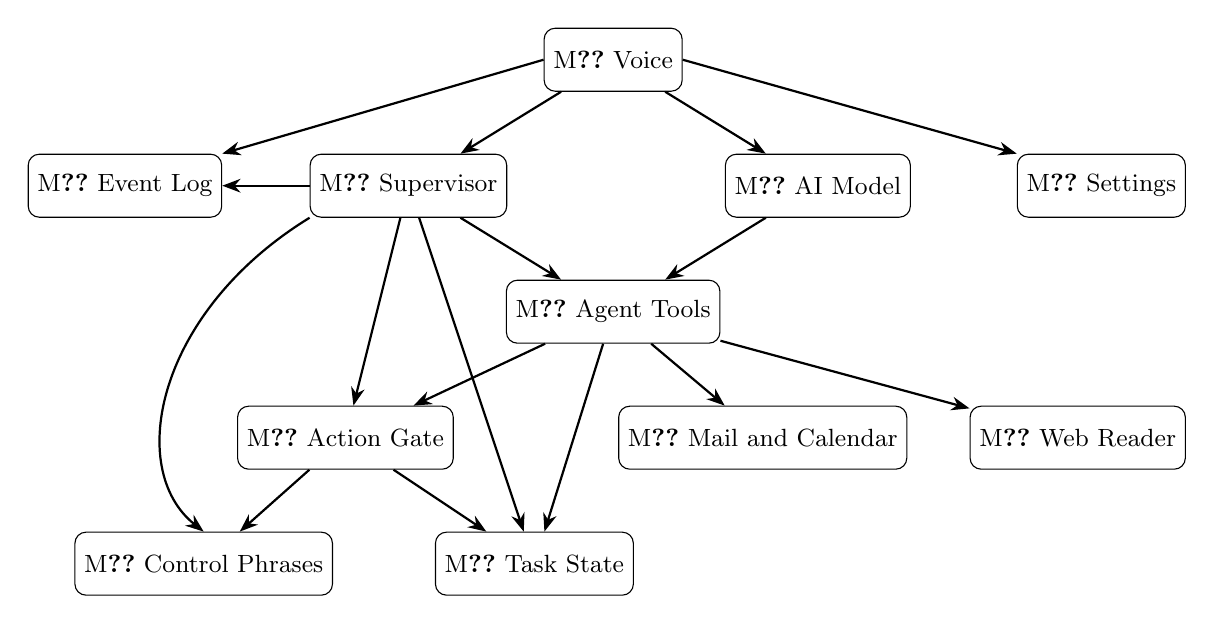
\begin{tikzpicture}[
  box/.style={draw, rounded corners, minimum height=0.8cm, font=\small, align=center},
  use/.style={-{Stealth}, thick}]
\node[box] (voice) at (0,0) {\mref{mVoice} Voice};
\node[box] (log) at (-6.2,-1.6) {\mref{mLog} Event Log};
\node[box] (sup) at (-2.6,-1.6) {\mref{mSupervisor} Supervisor};
\node[box] (ai) at (2.6,-1.6) {\mref{mAI} AI Model};
\node[box] (set) at (6.2,-1.6) {\mref{mSettings} Settings};
\node[box] (tools) at (0,-3.2) {\mref{mTools} Agent Tools};
\node[box] (gate) at (-3.4,-4.8) {\mref{mGate} Action Gate};
\node[box] (acc) at (1.9,-4.8) {\mref{mAccounts} Mail and Calendar};
\node[box] (web) at (5.9,-4.8) {\mref{mWeb} Web Reader};
\node[box] (phr) at (-5.2,-6.4) {\mref{mPhrases} Control Phrases};
\node[box] (task) at (-1.0,-6.4) {\mref{mTask} Task State};
\draw[use] (voice) -- (sup);
\draw[use] (voice) -- (ai);
\draw[use] (voice.east) -- (set.north west);
\draw[use] (voice.west) -- (log.north east);
\draw[use] (sup) -- (log);
\draw[use] (sup) -- (tools);
\draw[use] (sup) -- (gate);
\draw[use] (sup) -- (task);
\draw[use] (sup.south west) .. controls (-5.8,-3.2) and (-6.2,-5.2) .. (phr.north);
\draw[use] (ai) -- (tools);
\draw[use] (tools) -- (gate);
\draw[use] (tools) -- (acc);
\draw[use] (tools) -- (web);
\draw[use] (tools) -- (task);
\draw[use] (gate) -- (phr);
\draw[use] (gate) -- (task);
\end{tikzpicture}}
\caption{Use hierarchy among modules}
\label{FigUH}
\end{figure}

\todo{Check every arrow against the code once each owner has finished their module, and redraw if a module's uses change.}

\section{User Interfaces}

The user talks to the system and hears its replies. The web page (\mref{mClient}) offers the same controls by keyboard: start and end a session, stop, continue, cancel, approve and decline, and a text box. It shows the conversation and the task state. \todo{Lucas: add a sketch or screenshot of the page and the key bindings.}

\section{Design of Communication Protocols} \label{SecProtocols}

The client and the Voice Module meet in a LiveKit room. Audio flows both ways. The client sends commands as data messages on the topic \texttt{control} (stop, resume, cancel, approve, decline) and typed text on \texttt{lk.chat}. The Voice Module sends transcripts on \texttt{lk.transcription} and publishes the task state as the participant attribute \texttt{task\_state}. The client gets a short-lived room token from its own server route; the LiveKit secret never reaches the browser.

\section{Timeline} \label{SecTimeline}

\begin{table}[H]
\centering
\begin{tabular}{p{0.38\textwidth} p{0.2\textwidth} p{0.3\textwidth}}
\toprule
\textbf{Module} & \textbf{Owner} & \textbf{POC status (Nov 11)}\\
\midrule
\mref{mVoice} Voice & Lucas & Built; voice test pending\\
\mref{mClient} Accessible Client & Lucas & Built; VoiceOver check pending\\
\mref{mPhrases} Control Phrases & Lucas & Built and tested\\
\mref{mSupervisor} Supervisor & Aaron & Built and tested\\
\mref{mTask} Task State & Aaron & Built and tested\\
\mref{mGate} Action Gate & Aaron & Built and tested\\
\mref{mTools} Agent Tools & Aaron & Built and tested\\
\mref{mAI} AI Model & Aaron & Built; checked with the real model\\
\mref{mWeb} Web Reader & Aaron & Built; real browser untested in this version\\
\mref{mAccounts} Mail and Calendar & Curtis & Built and tested (made-up data)\\
\mref{mLog} Event Log & Kevin & Built and tested\\
\mref{mSettings} Settings & Kevin & Built\\
\bottomrule
\end{tabular}
\caption{Module owners and status}
\end{table}

\section*{Generative AI Use Disclosure}

\todo{Fill in as the rubric asks: the tools used and their versions, how and where each was used in this document, and how the content was checked. Each author adds their own part.}

\begin{thebibliography}{9}
\bibitem{Parnas1972} D. L. Parnas, ``On the criteria to be used in decomposing systems into modules,'' \emph{Communications of the ACM}, vol. 15, no. 12, pp. 1053--1058, 1972.
\bibitem{ParnasEtAl1984} D. L. Parnas, P. C. Clements and D. M. Weiss, ``The modular structure of complex systems,'' in \emph{Proc. 7th International Conference on Software Engineering}, 1984, pp. 408--417.
\end{thebibliography}

\end{document}
